\documentclass{article}
\usepackage[utf8]{inputenc}
\usepackage{subfig}
\usepackage{amsmath}

\usepackage{graphicx}
% \usepackage[legalpaper, landscape, margin=0.5cm]{geometry}
\usepackage[legalpaper, portrait, margin=0.5cm]{geometry}

\thispagestyle{empty}
% \renewcommand{\thesubfigure}{\roman{subfigure}}
\begin{document}

\begin{figure}[h]
        \centering
        % \subfloat[radiography]{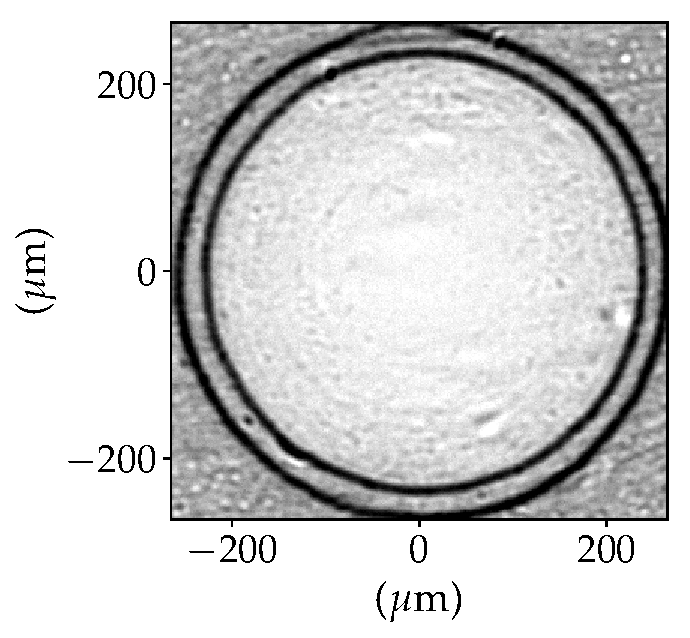
\includegraphics[height=4cm]{figures/ch04b/radio_workflow_a_FC_CDo01_these3.pdf}}\hspace{0.1cm}
        % \subfloat[cross-correlation map]{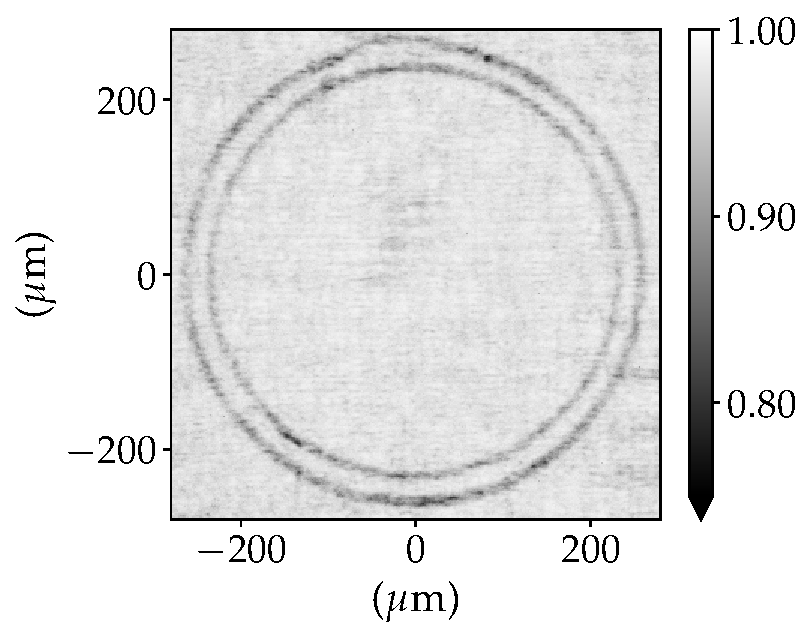
\includegraphics[height=4cm]{figures/ch04b/corr_max_2D_CDo01_these.pdf}}\\
        \subfloat[horizontal gradient $(\mu\text{rad})$]{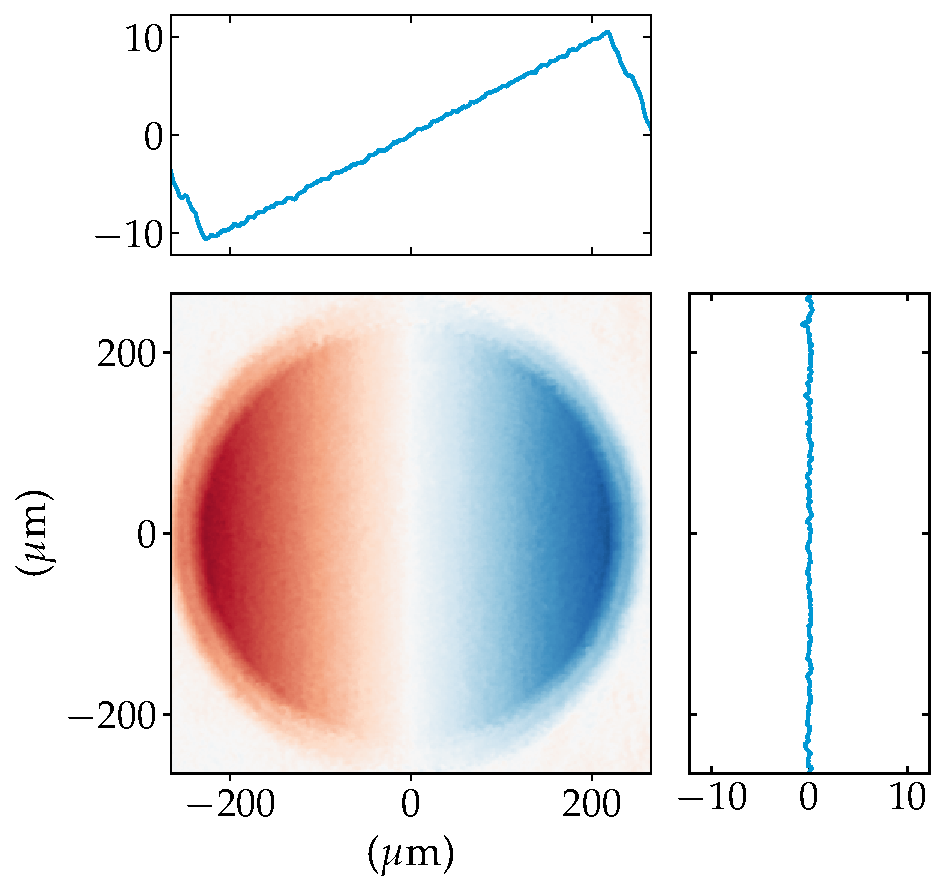
\includegraphics[height=5.07cm]{figures/ch04b/hor_grad_workflow_a_FC_CDo01_these3.pdf}}\hspace{0.1cm}
        \subfloat[vertical gradient $(\mu\text{rad})$]{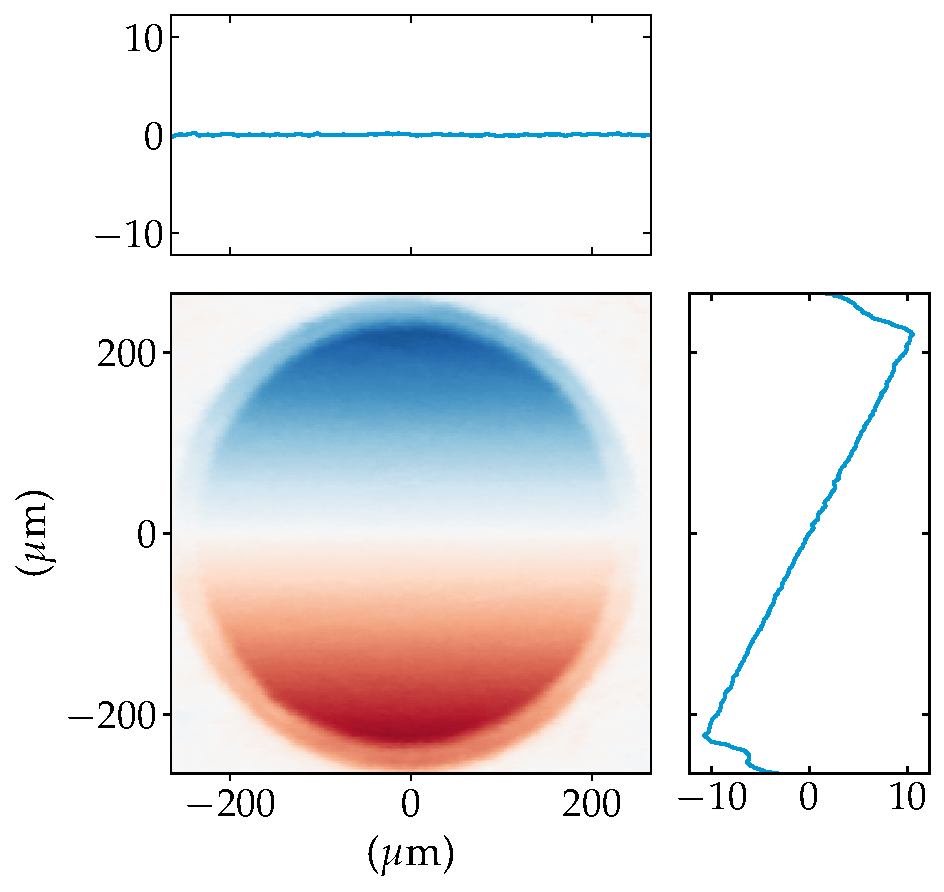
\includegraphics[height=5.07cm]{figures/ch04b/ver_grad_workflow_a_FC_CDo01_these3.pdf}}\\
        \subfloat[horizontal gradient residue $(\mu\text{rad})$]{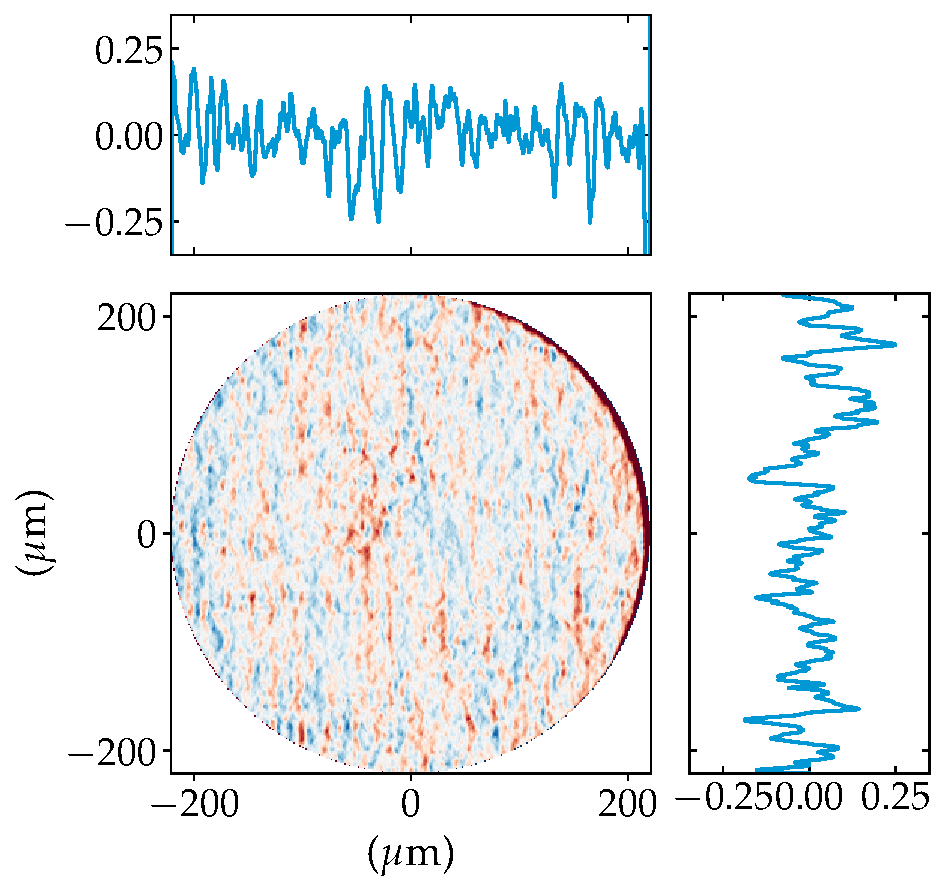
\includegraphics[height=5.07cm]{figures/ch04b/hor_grad_res_workflow_a_FC_CDo01_these3.pdf}}\hspace{0.1cm}
        \subfloat[vertical gradient residue $(\mu\text{rad})$]{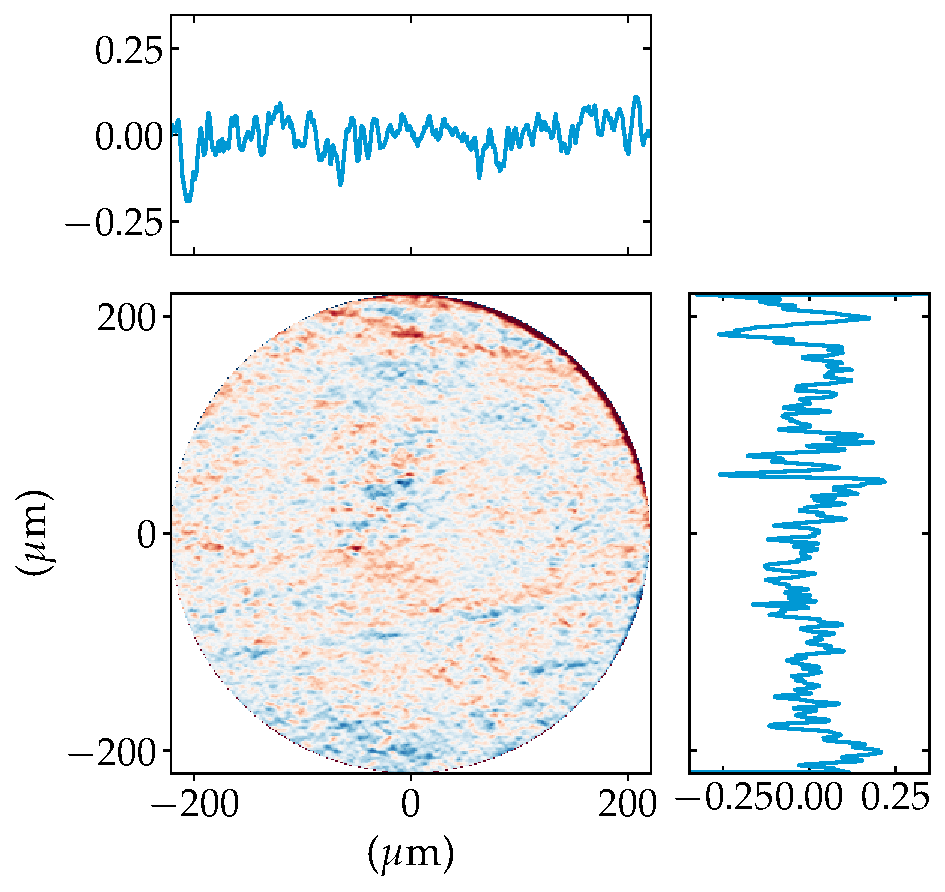
\includegraphics[height=5.07cm]{figures/ch04b/ver_grad_res_workflow_a_FC_CDo01_these3.pdf}}\\
\end{figure}
\end{document}